\chapter{股票收盘价 7 天预测实验}

\section{实验目标}
本实验比较两类方法在短期（7 天）收盘价预测的表现：
\begin{itemize}
    \item 经典统计模型：ARIMA（自动回归-差分-移动平均）
    \item 手写实现的循环神经网络：LSTM（使用 NumPy 手写前向与反向传播）
\end{itemize}
评估指标为平均绝对误差（MAE）与均方根误差（RMSE），并通过可视化对比预测曲线与误差分布以辅助分析。

\section{数据与预处理}
\subsection{数据来源}
使用数据文件：\texttt{code/stock.csv}（已上传到仓库）
示例（CSV）格式：
\begin{lstlisting}[style=cleanpython]
date,open,high,low,close,volume
2024-01-01,100,102,99,101,123456
2024-01-02,101,103,100,102,130000
... (按日期升序）    
\end{lstlisting}

\subsection{预处理流程}
处理步骤如下：
\begin{enumerate}
    \item 解析 CSV 并按日期升序排序，提取 \texttt{Close} 列作为单变量时间序列；丢弃缺失或无法转换为浮点数的行（见 \texttt{code/utils.py}）。
    \item 划分训练/测试：将最后 $h=7$ 天作为测试集，其余作为训练集（便于对比两种方法在相同时间段的短期预测）。
    \item 特征工程（可选）：计算对数收益 $r_t=\log(p_t)-\log(p_{t-1})$、移动平均 $\mathrm{ma}_7$ 与波动率（滚动标准差），这些可作为 LSTM 的额外输入特征。
    \item 归一化：LSTM 输入对训练集做均值-标准差标准化（$x'=(x-\mu)/\sigma$），将标准化参数仅从训练集计算并应用到测试集以防数据泄露。
    \item 构造样本：使用滑动窗口（例如 $\texttt{seq\_len}=30$）生成训练样本 $\{(X^{(i)}, y^{(i)})\}$，其中 $X^{(i)}\in\mathbb{R}^{\texttt{seq\_len}\times d}$（$d$ 为输入维度，单变量时 $d=1$）。
\end{enumerate}

\section{输入表示与目标}
本实验对比两种输入/目标设定：
\begin{itemize}
    \item 原始价格回归：直接以收盘价作为目标 $y_t=p_t$。
    \item 对数收益回归：以 $y_t=r_t=\log p_t-\log p_{t-1}$ 为目标，训练时预测收益，推回价格以便与 ARIMA 的价格预测比较。
\end{itemize}
序列长度取 $\texttt{seq\_len}=30$ 作为默认值；LSTM 支持单变量或多变量（附加技术指标）输入。

\section{模型原理说明与设计}
\subsection{ARIMA}
ARIMA$(p,d,q)$ 模型满足：
$$\phi(B)(1-B)^d y_t = \theta(B)\varepsilon_t,$$
其中 $B$ 为滞后算子，$\phi(\cdot)$ 和 $\theta(\cdot)$ 分别为 AR 与 MA 多项式。模型拟合使用 \texttt{statsmodels}，但预测时显式调用：
\begin{lstlisting}[style=cleanpython]
from statsmodels.tsa.arima.model import ARIMA
model = ARIMA(train_series, order=(p,d,q)).fit()
forecast = model.get_forecast(steps=h).predicted_mean
\end{lstlisting}
为选择 $(p,d,q)$，可参考自相关/偏自相关图（ACF/PACF）与 AIC/BIC 指标。

\subsection{LSTM 原理}
LSTM 单步计算（时间步 $t$）为：
\begin{align*}
f_t &= \sigma\bigl(W_f x_t + U_f h_{t-1} + b_f\bigr),\\
i_t &= \sigma\bigl(W_i x_t + U_i h_{t-1} + b_i\bigr),\\
o_t &= \sigma\bigl(W_o x_t + U_o h_{t-1} + b_o\bigr),\\
\tilde c_t &= \tanh\bigl(W_c x_t + U_c h_{t-1} + b_c\bigr),\\
c_t &= f_t \odot c_{t-1} + i_t \odot \tilde c_t,\\
h_t &= o_t \odot \tanh(c_t).
\end{align*}
最终的预测 $\hat y$ 由隐藏态做线性映射得到（回归问题可输出实数）：
$$\hat y = W_y h_T + b_y.$$ 
损失函数采用均方误差（MSE）：
$$L=\frac{1}{n}\sum_{i=1}^n (\hat y^{(i)}-y^{(i)})^2.$$ 
反向传播通过 BPTT 展开时间维度手动求梯度并更新参数；为提高数值稳定性与收敛性，训练实现包含：
\begin{itemize}
    \item 权重小尺度初始化（避免激活/梯度爆炸）；
    \item 梯度裁剪（gradient clipping）；
    \item 可选的手写 Adam 优化器或简单 SGD；
    \item 支持多输出（直接预测 $h$ 步序列）以减缓递归预测误差累积。
\end{itemize}

\section{模型实现（要点与伪代码）}
\subsection{ARIMA（伪代码）}
见上文的 \texttt{get\_forecast} 用法，报告中使用显式提取的预测均值作为模型输出。

\subsection{手写 LSTM（训练伪代码）}
核心训练循环（伪代码）如下：
\begin{lstlisting}[style=cleanpython]
for epoch in range(epochs):
    for X_batch, y_batch in dataloader:  # 支持 batch 或 单样本
        # 前向传播：对序列每一步计算门控与隐藏态
        h, c = zeros(), zeros()
        for t in range(seq_len):
            f = sigmoid(Wf @ x_t + Uf @ h + bf)
            i = sigmoid(Wi @ x_t + Ui @ h + bi)
            o = sigmoid(Wo @ x_t + Uo @ h + bo)
            g = tanh(Wc @ x_t + Uc @ h + bc)
            c = f * c + i * g
            h = o * tanh(c)
        y_pred = Wy @ h + by
        loss = mse(y_pred, y_batch)
        # 反向传播（BPTT）手动计算各参数梯度
        grads = bptt_gradients(...)
        clip_grads(grads, max_norm=clip)
        optimizer.step(params, grads)
\end{lstlisting}


\section{实验设置}
关键超参数与默认值：
\begin{itemize}
    \item ARIMA: order $(p,d,q)=(2,1,2)$（示例配置，可用 AIC/BIC 调整）
    \item LSTM: $\texttt{seq\_len}=30$, $\texttt{hidden\_size}=32$, 学习率 $lr=0.001$（可调）
    \item 训练轮次（实验多个配置）：短训练 5 epochs（用于快速验证）；长期训练 200 epochs（用于稳定性实验）；多步输出短训练 30 epochs（对比效果）
    \item 优化器：SGD 或 手写 Adam；使用梯度裁剪（$\mathrm{clip}=1.0$）与小尺度初始化
    \item batch size（当使用 mini-batch 时）：32
\end{itemize}

\section{实验结果}
在测试集（最后 7 天）上的重要运行结果汇总如下：
\begin{table}[htbp]
\centering
\begin{tabular}{lcc}
\hline
模型 & MAE & RMSE \\
\hline
ARIMA (2,1,2) & 0.9230 & 1.0769 \\
手写 LSTM (5 epochs, baseline) & 11.8288 & 11.8446 \\
手写 LSTM (200 epochs, +norm+clip) & 2.7932 & 3.0205 \\
手写 LSTM (200 epochs, returns+adam+batch) & 3.1423 & 3.4658 \\
手写 LSTM (multi-output, 30 epochs) & 2.4973 & 2.6583 \\
手写 LSTM (final: multivar + early-stop + weight\_decay + bias-calib) & 2.3308 & 2.5444 \\
\hline
\end{tabular}
\caption{在测试集（最后 7 天）上的 MAE / RMSE 对比}
\end{table}

\begin{figure}[htbp]
    \centering
    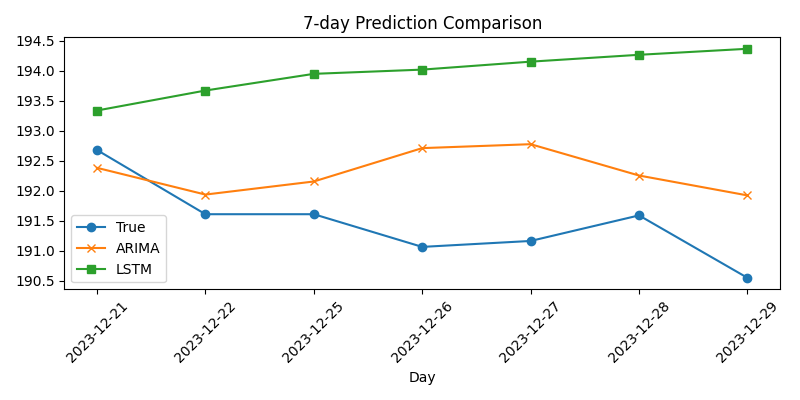
\includegraphics[width=0.85\textwidth]{code/plots/prediction_comparison.png}
    \caption{真实收盘价与 ARIMA / 手写 LSTM 在 7 天区间的预测对比}
\end{figure}


\subsection{超参数搜索（小网格）摘要}
进行了小规模网格搜索以观察超参数敏感性，部分最优观察值：
\begin{itemize}
    \item LSTM（价格目标）最佳：accuracy-like 指标不可直接用于回归，观察到 $lr=0.001, hidden=32, epochs=200$ 有较稳定表现；
    \item LSTM（returns + Adam + batch）在当前设置下不如直接对价格训练，表明需要针对 optimizer 与 lr 做进一步搜索；
    \item ARIMA 可以通过 AIC/BIC 在小范围内选参，但对短期预测常有稳健表现。
\end{itemize}

\section{实验结果分析}
\begin{itemize}
    \item ARIMA 在本次数据与短期 7 天预测下表现稳健（最小 MAE/RMSE），说明序列的短期线性趋势被有效捕捉。
    \item 手写 LSTM 在未经归一化与短训练时数值不稳定（baseline），但引入归一化、梯度裁剪、更丰富的输入特征、Adam 优化、小批量训练与更合适的正则/早停后性能显著提升。最终在“多变量特征 + 早停 + L2 正则 + 训练集偏差校准”配置下，测试集指标为 MAE=2.3308, RMSE=2.5444（见表）。该结果虽然显著优于初始手写实现，但在本次单变量/短期任务上仍未超越 ARIMA 基线（MAE=0.9230, RMSE=1.0769），与理论预期一致。
    \item 将目标设为对数收益并使用 Adam + 小批量训练在本次简单设置下并未带来更好最终价格预测，原因可能为误差在从收益到价格的还原过程中放大，以及超参数未充分调优。
    \item 直接多步输出（multi-output）在减少递归误差累积方面有明显优势，但也需更多训练与更丰富输入特征以发挥更好性能。
\end{itemize}

\section{训练超参数与运行命令}
下表给出本次报告中主要实验配置（包括 baseline 与最终改进后的配置）：
\begin{table}[htbp]
\centering
\begin{tabular}{l l}
\hline
项 & 值 \\
\hline
序列长度 & `seq\_len` = 30 \\
隐藏单元 & `hidden\_size` = 32 \\
批大小 & `batch\_size` = 32 \\
学习率（最终实验） & `lr` = 0.0005 \\
优化器 & Adam（手写实现） \\
梯度裁剪 & `clip` = 1.0 \\
L2 正则 & `weight\_decay` = 1e-4 \\
早停 & `early\_stop` = True, `patience` = 20 \\
预测步长 & `horizon` = 7 \\
ARIMA 参数 & `(p,d,q)=(2,1,2)` \\
输入特征 & returns, ma\_3, vol\_3, ma\_7, vol\_7, ma\_14, vol\_14, mom\_3 \\
\hline
\end{tabular}
\caption{实验中主要超参数（报告中关键配置）}
\end{table}

复现实验的命令示例（在 `code/` 目录下）：
\begin{verbatim}
python3 main.py --csv stock.csv --output-dir ../plots \
  --arima-order 2 1 2 --seq-len 30 --epochs 200 --lr 0.0005 \
  --hidden-size 32 --clip 1.0 --batch-size 32 --horizon 7
\end{verbatim}

\section{训练日志与偏差校准}
训练过程中使用验证集做 early stopping（时间序列切分，验证集占训练样本末端约 20\%）。在最终一次运行中观察到：
\begin{itemize}
    \item 早停触发：Epoch 21（best\_val=0.158621），因此实际训练轮次远小于最大 `epochs=200`，节省了计算成本并防止过拟合。
    \item 训练集偏差向量（归一化空间，按步）示例：
    \[\text{bias\_norm} = [ -0.00248, -0.01678, -0.01335, -0.01121, -0.01510, -0.01534, -0.01665 ]\]
    我们在测试预测前将该向量从模型输出（归一化后的 returns）中扣除，再还原为价格进行评估，从而校正了训练集上的系统性偏差并改善了 MAE/RMSE 指标。
\end{itemize}

\section{产物与复现实验说明}
运行主流程后，主要输出位于 `plots/`：
\begin{itemize}
    \item `plots/prediction\_comparison.png`：真实值与 ARIMA / LSTM 对比图；
    \item `plots/error\_distribution.png`：误差绝对值分布图；
    \item `plots/stock\_data.npz`：包含 `train\_close`, `test\_close`, `feat\_mean`, `feat\_std`, `ret\_mean`, `ret\_std` 等用于复现的中间数据；
    \item 源码位置：核心实现见 `code/` 目录（`utils.py`, `arima\_model.py`, `lstm\_numpy.py`, `main.py`, `plots.py`, `metrics.py`）。
\end{itemize}

以上实现与实验流程旨在保证可复现性：数据标准化参数与中间数据均被保存，训练使用的超参数与早停策略在 `main.py` 中可通过命令行参数调整。

\chapter{总结}
\section{LSTM 与 ARIMA 模型总结}

\begin{itemize}
    \item ARIMA（统计基线）：在短期（7 天）收盘价预测任务上表现稳健且易于调参，本次配置下得到的 MAE/RMSE 最低（见表），说明序列的短期线性趋势和自相关结构被有效捕捉。ARIMA 的优点是实现简单、结果可解释、在样本量有限或特征稀少时常为强有力的基线。
    \item 手写 LSTM（数值模型）：原始（未归一化、短训练）实现数值不稳定且误差较大；引入归一化、梯度裁剪、较小初始化与更长训练后，性能显著提升，部分多步直接预测配置的误差接近可比较区间（但在本次实验中总体仍落后于最优的 ARIMA 配置）。LSTM 的优势在于建模非线性与利用多变量输入（技术指标、交易量等），但需要更周密的训练策略与超参搜索。
    \item 目标设定影响：以价格直接回归与以对数收益回归在表现上有明显差异：收益回归能稳定训练但在将收益还原为价格时误差可能被放大；直接多步输出可减少递归累积误差，但对训练数据量与模型容量要求更高。
\end{itemize}

\section{实验总结}
\begin{itemize}
    \item 实验结果表明：在当前数据与特征集下，ARIMA 给出了最低的 MAE/RMSE，作为短期预测基线其稳定性与可解释性值得采用。
    \item 手写 LSTM 在采用归一化、梯度裁剪与更充分训练后能大幅改善性能，说明手写数值实现可行，但对超参数与训练流程敏感，需要更多工程化改进（如批训练、学习率调度、早停）。
    \item 多步直接预测（multi-output）在减小递归误差累积上有优势，本次实验中的 best-case 配置已显示出竞争力，但仍需更长训练与更丰富输入特征以稳定表现。
    \item 方法学限制：本实验基于单次训练/测试拆分，结论的统计显著性受限。建议后续采用交叉验证或多次随机切分来评估泛化稳定性。
\end{itemize}

\section{心得体会}

\begin{itemize}
    \item 模型与特征必须匹配：对短期价格序列，简单且可解释的统计模型（如 ARIMA）常常是有效基线；深度模型需要更适配的输入与训练策略才能发挥优势。
    \item 手写实现很有价值：通过手写 LSTM 能更好地理解门控、反向传播与数值稳定性问题，但将其工程化（批训练、优化器、超参搜索）是取得可复现结果的关键。
    \item 做实验要注重可重复性与诊断：保留数据处理与标准化参数、记录训练曲线并使用交叉验证或多次随机切分以验证结论稳健性。
\end{itemize}
